%\subsubsection{Water}
%The goal of this section is to use equation \ref{t2eq} to determine $T_{2}^*$ for water, alcohol and rubber. Let's first explore how to determine $T_{2}^*$ for water. The raw signal for water is shown below in Figure 4:

%\begin{figure}[H]
%\centering
%\label{fidwater1}
%\includegraphics[width=0.6\textwidth]{FIDwatertotalSig.jpg}
%\caption{Complete oscilloscope trace for the FID of water.}
%\end{figure}
%
%\begin{figure}[H]
%\centering
%\label{fidwater1}
%\includegraphics[width=0.6\textwidth]{FIDshiftedWater.jpg}
%\caption{FID of water where the initial noise from the detector is removed and the signal is shifted up so that the exponential approaches 0.}
%\end{figure}

%First, the voltage values were shifted up so that the signal approached 0. This is important because equation \ref{t2eq} approaches 0 as time approaches infinity. Hence, if this was not done any resulting analysis would not be as accurate. Next, we decided to only analyze the data that proceeded after the start of a smooth exponential decay. Often, there was a larger voltage spike or other noise that occurred before the start of the exponential decay. This can be caused by the ringing effect of the detector circuit. After the signal was shifted and beginning noise was discarded, as shown above in Figure 5, we approximated $T_{2}^*$ using the following manipulation of equation \ref{t2eq}:

%\begin{align*}
%\text{if:} \\
%(t) &= \frac{M_0}{e} \\
%\text{then}: \\
%ln(\frac{1}{e}) &= ln(e^{\frac{-t}{T_{2}^*)}} \\
%-1 &- \frac{-t}{T_{2}^*} \\
%t &= T_{2}^* 
%\end{align*}

%Therefore, we can approximate $T_{2}^*$ by finding the \textit{t} value where $M(t) \approx \frac{M_0}{e}$. This is shown in the graph below:

\begin{figure}[H]
\centering
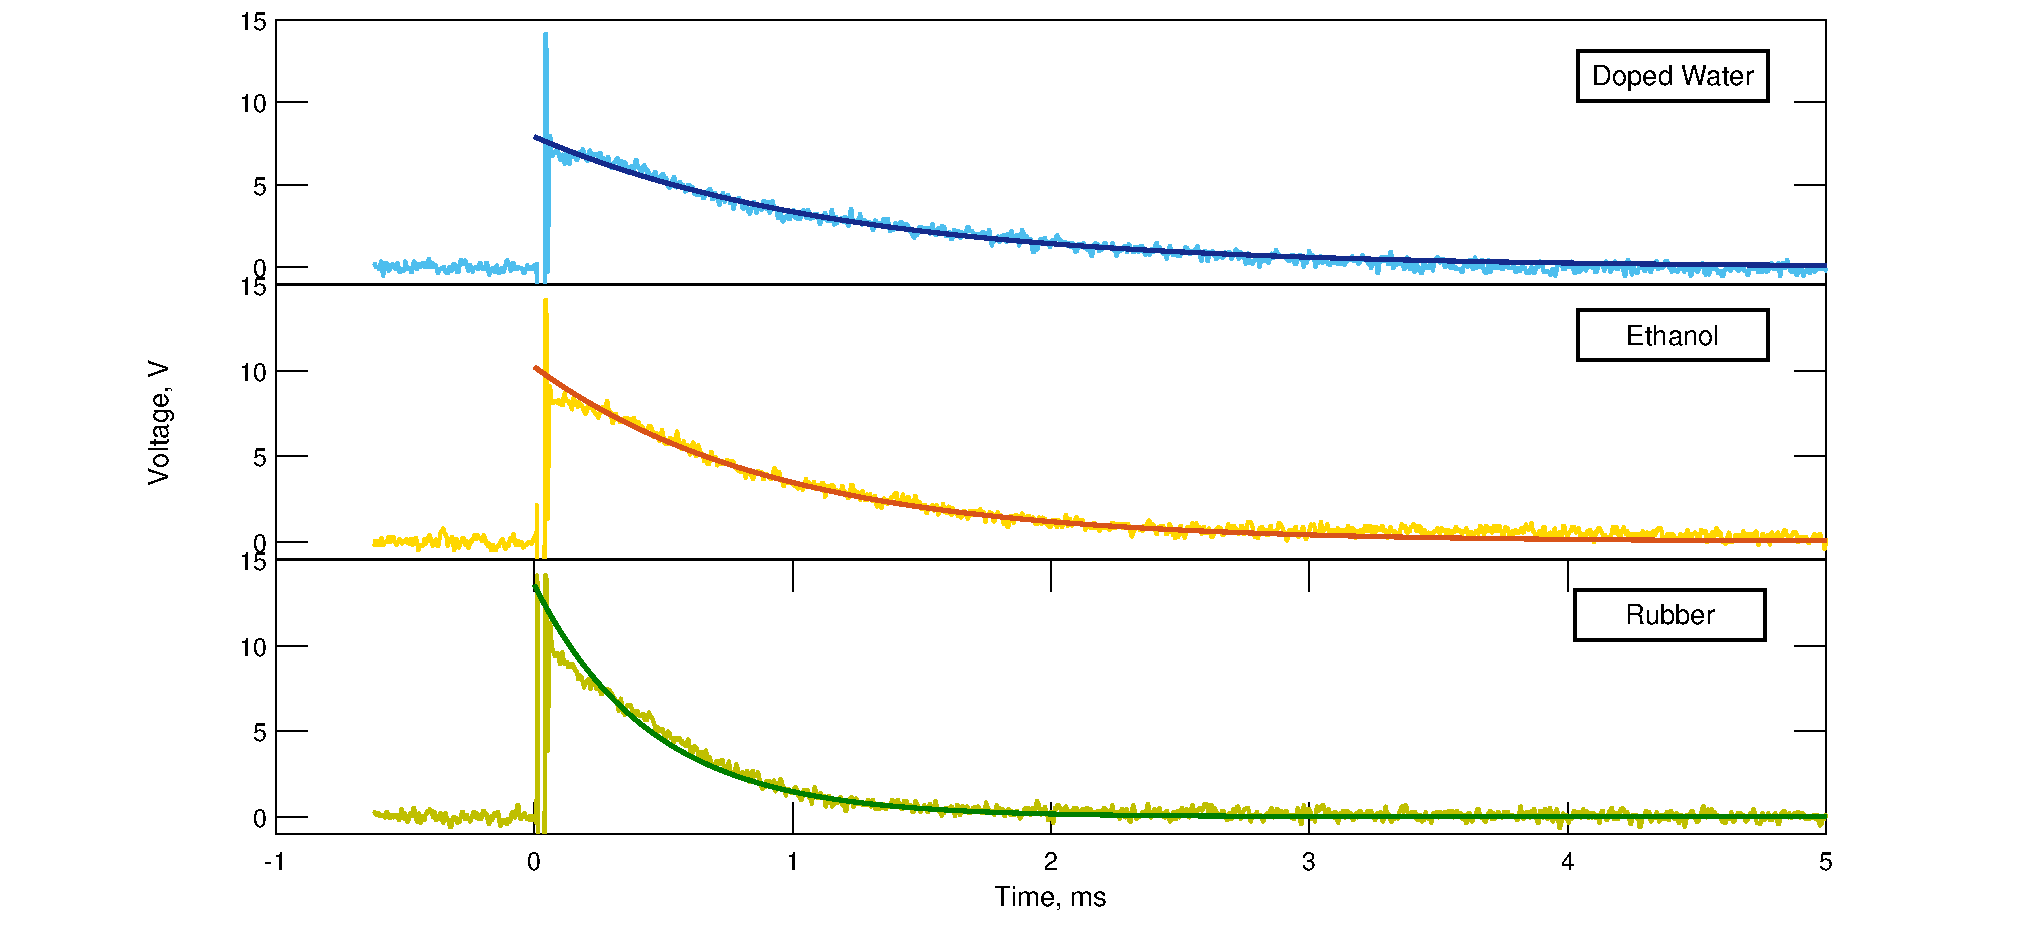
\includegraphics[width=\textwidth]{figures/B2/B2_1.eps}
\caption{Water $T_2^* = 1.169 \pm 0.017$, Ethanol $T_2^* = 0.9239 \pm 0.0085$, Rubber $T_2^* = 0.4495 \pm 0.0073$ }
\label{fig:B2:T2samples}
\end{figure}

%Using the figure above, we can deduce that $T_{2}^*$ is approximately $1.09\times 10^{-3}$ s. Due to the noise fluctuations, it was hard to determine the value for $M_0$. Around the peak of the signal the highest point of the noise was 0.770 V and the lowest was 0.689 V. The average $M_0$ divided by \textit{e} is therefore approximately 0.27 V. However, the noise isn't as evenly distributed near the peak so taking the average isn't as ideal. Given that the range between the maximum and minimum is 0.08 V, it seems reasonable to estimate the uncertainty of $M_0$ to be $\pm 0.05$ V (a bit larger than half because the noise was not as evenly distributed). The closest corresponding data point is at 0.274 V. The range of time values where the voltage is 0.274 V is $9.34\times 10^{-4}$ s to $1.23\times 10^{-3}$ s. Therefore, taking the average again, $T_{2}^*$ is approximately $1.08\times 10^{-3}$ s. The uncertainty was approximated by taking half of the range between the maximum and minimum. The result was an uncertainty of $\pm 2 \times 10^{-4}$ s. Therefore, $T_{2}^*$ is approximately $(1.1\times 10^{-3} \pm 2 \times 10^{-4})$ s using this method. To obtain a more precise value for $T_{2}^*$, MATLAB's \textit{fit} function was used to fit the data to an exponential of the form:

%\begin{align*}
%y &= ae^{bx}
%\end{align*}

%Below is a graph of the fit:

%\begin{figure}[H]
%\centering
%\label{expFitWater}
%\includegraphics[width=0.6\textwidth]{FIDWaterExp.jpg}
%\caption{FID graph for water showing the exponential fit.}
%\end{figure}

%As you can see in the above figure, the fit was fairly accurate.The coefficients from the \textit{fit} function for above fit were:

%\begin{align*}
%   a &=      (0.846 \pm 0.005) \text{ V} \\
%       b &=       (-1046 \pm 8) \text{ s}^{-1}
%\end{align*}

%To see the impact of smoothing the data, a Savitzky-Golay filter was used. A Savitzky-Golay filter aims to increase the signal to noise ratio using convolution by fitting successive subsets of adjacent data points with a low-degree polynomial by the method of linear least squares. Below is the result of the filter and new fit:

%\begin{figure}[H]
%\centering
%\label{expFitWater3}
%\includegraphics[width=0.6\textwidth]{FIDfilteredWaterExp.jpg}
%\caption{Water FID graph showing the exponential fit for the filtered data.}
%\end{figure}

%The fit is similar to Figure 6. The coefficients of the MATLAB \textit{fit} function for the above filtered data were:

%\begin{align*}
%    a &=      (0.846 \pm 0.003) \text{ V} \\
%       b &=       (-1046  \pm 4) \text{ s}^{-1} \\
%\end{align*}
      
%It is very reassuring that after applying the filter, the precision of the fit coefficients increased but the coefficient values remained the same. As a result, we know that for this data set, the filter is not impacting the behaviour of the original signal. Equation \ref{t2eq} was used to approximate $T_{2}^*$. From equation \ref{t2eq}, we know that:
%\begin{align*}
%b &= \frac{-1}{T_{2}^*} \\
%\text{Therefore:} \\
%T_{2}^* &= \frac{-1}{b} \\
%\text{from the fit we know that:} \\
%b&= -1046 \text{s}^-1 \\
%\text{Therefore:} \\
%T_{2}^* &\approx 9.56 \times 10^{-4} \text{s} 
%\end{align*}

The uncertainty for $T_{2}^*$, $\Delta T_{2}^*$, can be approximated as follows:
\begin{align*}
\Delta T_{2}^* &= \frac{\Delta b}{\left| b \right|} \times T_{2}^* \\
\Delta T_{2}^* &= \frac{4}{1046} \times 9.56 \times 10^{-4} \text{s} \\
\Delta T_{2}^* &= \pm 4 \times 10^{-6} \text{s}
\end{align*}

%Therefore, the approximation for $T_{2}^*$ using an exponential fit is $(9.56 \times 10^{-4} \pm 4 \times 10^{-6}) \text{s}$. 

%We will now explore plotting the data on a semi log graph to determine $T_{2}^*$. If we take the ln of both sides of equation \ref{t2eq} we get:

\begin{align}
\label{fun}
ln(M(t)) &= lnM_0 -\frac{t}{T_{2}^*}
\end{align}

%As before, the data values for this section were the shifted values in Figure 5. The signal was also clipped as soon as the voltage became negative so that the ln of the voltage could be calculated. It was also noticed that the ln of the signal started to become more noisy as the signal approached 0. The ln of the voltage values vs. the time was plotted and the MATLAB function \textit{fitlm} was used to perform the linear regression. The results are shown in the figure below:

%\begin{figure}[H]
%\centering
%\label{linWater1}
%\includegraphics[width=0.6\textwidth]{FIDWaterLn1.jpg}
%\caption{Linear fit for the ln of the voltage vs. time graph for water.}
%\end{figure}

The \textit{fitlm} function outputted a slope of $(-1038 \pm 7) \text{s}^{-1}$ and an intercept of $-0.175 \pm 0.005$. The $\text{R}^2$ of the fit was 0.971. \\

Equation \ref{fun} was used to solve for $T_{2}^*$:

\begin{align*}
m &= \frac{-1}{T_{2}^*} \\
T_{2}^* &= \frac{-1}{m} \\
T_{2}^* &= \frac{-1}{-1038} \\
T_{2}^* &= 9.63 \times 10^{-4} s \\
\end{align*}

The uncertainty for $T_{2}^*$ was calculated using the same method that was used for calculating its uncertainty for the exponential fit approach. Therefore, the approximation for $T_{2}^*$ using an linear fit is $(9.63 \times 10^{-4} \pm 6 \times 10^{-6}) \text{s}$. 

To see if we could get a more accurate fit, we applied the linear regression to the ln of the filtered data from above. The results are shown below:

%\begin{figure}[H]
%\centering
%\label{linWater2}
%\includegraphics[width=0.6\textwidth]{FIDLnWaterFilter.jpg}
%\caption{Linear fit for the ln of the voltage vs. time graph for filtered data for water.}
%\end{figure}

%The \textit{fitlm} fit outputted a slope of $(-972.67 \pm 2) \text{s}^{-1}$ and an intercept of $-0.207 \pm 0.003$. The $\text{R}^2$ of the fit was 0.9995. Using the method outlined above, $T_{2}^*$ for this fit was approximately $(1.028 \times 10^{-3} \pm 2 \times 10^{-6}) \text{s}$. Both the $\text{R}^2$ value and the level of precision of the coefficients improve after filtering the data but the slope differs from the slope of fit using the raw data which is concerning. The slopes differ by about 6\% which is not outrageous but is not negligible either. At the very least, the filtering better illustrates how well the filtered data matches the fit. From Figure 10 above, we can see that the fit alternates from overestimation to underestimation when compared to the filtered data. This could be a sign that there is a small frequency difference between our sample and the detector circuit. This would cause a slight beat in our signal. 


%\subsubsection{Ethanol} 

%The graph of the complete signal for ethanol is shown below:

%\begin{figure}[H]
%\centering
%\label{linWater2}
%\includegraphics[width=0.6\textwidth]{FIDEthanolFull.jpg}
%\caption{Complete oscilloscope trace for the FID of ethanol.}
%\end{figure}

%The graph of the shifted data with the initial detector noise removed is shown below:
%\begin{figure}[H]
%\centering
%\label{linWater2}
%\includegraphics[width=0.6\textwidth]{FIDEthShifted.jpg}
%\caption{FID of ethanol where the initial noise from the detector is removed and the signal is shifted up so that the exponential approaches 0.}
%\end{figure}

%$T_{2}^*$ for ethanol was first roughly approximated using the first estimation method that was used for water, with $M_0 \approx 0.634$ V. The $T_{2}^*$ value obtained using this method was $(1.25 \times 10^{-3} \pm 2 \times 10^{-4})$ s. Next, the ln approach for calculating $T_{2}^*$ for water was used for ethanol.\\

%The MATLAB \textit{fitlm} function was used to fit the ln of the voltage vs. the time using data shown above in Figure 12. The fit is shown below:
%\begin{figure}[H]
%\centering
%\label{linWater2}
%\includegraphics[width=0.6\textwidth]{FIDEthLn.jpg}
%\caption{Linear fit for the ln of the voltage vs. time graph for filtered data for water.}
%\end{figure}

%The output of the \textit{fitlm} function was a slope of -941 $s^{-1}$ $\pm$ 7 $s^{-1}$ with a y-intercept of -0.354 $\pm$ 0.006. The R-squared value for the fit is 0.862. Using the approach used for water, $T_{2}^*$ is approximately $(1.063 \times 10^{-3} \pm 8 \times 10^{-6}) \text{s}$.

%A Savitzky-Golay filter was applied to the data shown in Figure 12. Below is the result of applying \textit{fitlm} to the ln of the filtered data:
%\begin{figure}[H]
%\centering
%\label{ethanolFilteredLn}
%\includegraphics[width=0.6\textwidth]{FIDEthLnFiltered.jpg}
%\caption{Linear fit for the ln of the voltage vs. time graph for filtered data for water.}
%\end{figure}

%The output of the \textit{fitlm} function was a slope of -940 $s^{-1}$ $\pm$ 3 $s^{-1}$ with a y-intercept of -0.353 $\pm$ 0.003. R-squared value for the fit is 0.991. Using the approach used for water, $T_{2}^*$ is approximately $(1.064 \times 10^{-3} \pm 3 \times 10^{-6}) \text{s}$.For this data, the filter was very successful at filtering the data because the slope of the fit for the filtered data was very close to the slope of the fit for the raw data. In addition, filtering the data improved both the precision and the $\text{R}^2$ value. However, the fit deviates from the data, especially near the beginning of the signal. It could be the case that there is a more pronounced frequency difference between our sample and detector. Figures 11 and 12 illustrate that the signal bounces a tiny bit, as it goes below 0 and then increases a bit before leveling out.  

%\subsubsection{Rubber} 

%The graph of the complete signal for rubber is shown below:
%\begin{figure}[H]
%\centering
%\label{linWate}
%\includegraphics[width=0.6\textwidth]{FIDRubFull.jpg}
%\caption{Complete oscilloscope trace for the FID of rubber.}
%\end{figure}


%The graph of the shifted data with the initial detector noise removed is shown below:
%\begin{figure}[H]
%\centering
%\label{linWater2}
%\includegraphics[width=0.6\textwidth]{FIDRubShifted.jpg}
%\caption{FID of rubber where the initial noise from the detector is removed and the signal is shifted up so that the exponential approaches 0.}
%\end{figure}

%$T_{2}^*$ for rubber was first approximated using the estimation method that was used for water, with $M_0 \approx 1.05$ V. The $T_{2}^*$ value obtained using this method was $(6.13 \times 10^{-4} \pm 2  \times 10^{-5})$ s. Next, the ln approach for calculating $T_{2}^*$ for water and ethanol was used for rubber.\\

%The MATLAB \textit{fitlm} function was used to fit the ln of the voltage vs. the time using data shown above in Figure 16. The fit is shown below:
%\begin{figure}[H]
%\centering
%\label{linWater2}
%\includegraphics[width=0.6\textwidth]{FIDRubLn.jpg}
%\caption{Linear fit for the ln of the voltage vs. time graph for rubber.}
%\end{figure}

%The output of the \textit{fitlm} function was a slope of -1950 $s^{-1}$ $\pm$ 13 $s^{-1}$ with a y-intercept of 0.250 $\pm$ 0.008. R-squared value for the fit is 0.978. Using the approach used for water, $T_{2}^*$ is approximately $(5.13 \times 10^{-4} \pm 3 \times 10^{-6}) \text{s}$.


%A Savitzky-Golay filter was applied to the data shown in Figure 16. Below is the result of applying \textit{fitlm} to the ln of the filtered data:
%\begin{figure}[H]
%\centering
%\label{linWater2}
%\includegraphics[width=0.6\textwidth]{FIDRubLnFiltered.jpg}
%\caption{Linear fit for the ln of the voltage vs. time graph for filtered data for rubber.}
%\end{figure}

%The output of the \textit{fitlm} function was a slope of -1939 $s^{-1}$ $\pm$ 8 $s^{-1}$ with a y-intercept of 0.247 $\pm$ 0.005. R-squared value for the fit is 0.99. Using the approach used for water, $T_{2}^*$ is approximately $(5.16 \times 10^{-4} \pm 2 \times 10^{-6}) \text{s}$. For this data, the filter was fairly successful at filtering the data because there is about a 0.5\% difference between the slope of the fit for the filtered data and the slope of the fit for the raw data. In addition, filtering the data improved both the precision and the $\text{R}^2$ value.






\begin{table}[H]
    \centering
    \begin{tabular}{c|c}
    \toprule
        \textbf{Sample} & $T_1$ (ms) \\ \midrule
        {Doped Water} & $15.9725 \pm 1.2243$ \\
        {Ethanol} & $1031.8\pm 80.0$  \\
        {Rubber} & $27.3784 \pm 5.5746$ \\ \bottomrule
    \end{tabular}
    \caption{$T_1$ values for three samples, measured using a $90\degree-90\degree$ pulse sequence.}
    \label{tab:B3:T1values}
\end{table}


For example, with doped water (Figure \ref{fig:B3:example_uncertainty}), the time-delay for the three traces are,
\begin{align*}
    &\tau_1 = 10.2227\ \text{ms}, & &\tau_2 = 11.0175\ \text{ms}, & &\tau_3 = 11.9737\ \text{ms}
\end{align*}
\begin{align*}
    \tau &=  \frac{1}{3} \sum_{i=1}^3 \tau_i = 11.0713\ \text{ms} \\
    \Delta\tau &= \text{max}\left( |\tau - \tau_i | \right) = 0.8486 \ \text{ms}
\end{align*}


So, from Equation \ref{eqn:B3:T1} we can determine $T_1$ as,
\begin{align*}
    T_1 &= \frac{11.0713\pm0.8486}{\ln 2} \\
    &= 15.9725 \pm 1.2243 \ \text{s}
\end{align*}


\begin{align*}
    \tau &= \frac{1}{3} \sum_{i=1}^3 \tau_i\\
    \Delta \tau &= \text{max}\left( |\tau - \tau_i | \right)
\end{align*}
